%% JAIR Manuscript - Clement Frassier
%% Federated Learning: Principles and Implementation
%% Nurse Stress Detection (HEART Project)
%% English translation of rapport_acc_nouveau_.tex

\documentclass{article}
\usepackage{amsmath, amssymb}
\usepackage{booktabs}
\usepackage{graphicx}
\usepackage{hyperref}
\usepackage{xcolor}

%\setcopyright{cc}
%\acmDOI{10.1613/jair.1.xxxxx}

%\JAIRAE{Clement Frassier}
%\JAIRTrack{Applications}
%\acmVolume{4}
%\acmArticle{6}
%\acmMonth{8}
%\acmYear{2026}

\RequirePackage[
  datamodel=acmdatamodel,
  style=numeric,
  backend=biber,
  giveninits=true,
  uniquename=init
  ]{biblatex}

\renewcommand*{\bibopenbracket}{(}
\renewcommand*{\bibclosebracket}{)}

\addbibresource{sample-base.bib}

\begin{document}

\title[Federated Learning - Stress Detection]{Federated Learning: Principles and Implementation}

\author{Clement Frassier}
\orcid{0009-0000-0000-0000}
\email{clement.frassier@gmail.com}
\affiliation{%
  \institution{UKM / UEL}
  \city{Kuala Lumpur}
  \country{Malaysia}
}

\begin{abstract}
{\bf Background:}
Physiological data collected via connected wristbands in hospital settings constitute
personal health data subject to the GDPR~\cite{gdpr2016}. Aggregating them on a
central server exposes patients and staff to major re-identification risks, making
classic centralized approaches unsuitable in this context.

{\bf Objectives:}
We aim to train an automatic stress-detection model on data distributed across 15
nurses, without ever transmitting this data to a central server, while providing a
formal differential-privacy guarantee and producing a model deployable on an embedded
wristband (TinyML).

{\bf Methods:}
We propose a federated learning pipeline combining FedProx ($\mu = 0{,}05$) for
Non-IID heterogeneity, and DP-SGD via Opacus for $(\varepsilon, \delta)$-DP
differential privacy. The MLP Tiny model (1~362 parameters, 5.32~KB) is trained over
30 communication rounds and dynamically quantized to INT8 for deployment. A grid
search over 25 federated runs (5 values of $\sigma \in [0.6,\, 1.8]$, 5 independent
seeds) empirically measures the privacy/utility trade-off, compared against an
unconstrained centralized baseline (same model, same 5 seeds, no FL, no DP). This
baseline serves as a theoretical reference ceiling, not deployable in practice on
this type of health data under the GDPR, but useful for honestly quantifying the
cost of privacy.

{\bf Results:}
On a pooled test set (all nurses combined), the federated model reaches an accuracy
of $82.0 \pm 0.5\,\%$ on average over the 5 values of $\sigma$, versus
$81.95 \pm 0.89\,\%$ for the centralized model: statistically indistinguishable raw
accuracies. On class-balanced metrics, the centralized model retains an apparent
advantage ($57.8 \pm 1.2\,\%$ balanced-accuracy versus $\approx 47.9\,\%$ for FL). But
11 of the 15 nurses have a single-class test set, where a constant prediction
mechanically achieves $100\,\%$. These clients dominate the pooled result and mask
its true meaning. Restricted to the 4 clients with a genuinely mixed test set, the
most clinically honest measure, the gap shrinks sharply ($45.7 \pm 1.5\,\%$ for the
centralized model versus $42.7 \pm 1.0\,\%$ for FL), and the \textbf{centralized model
itself collapses}: its AUC-ROC drops to $0.267$ (below chance level), and its optimal
decision threshold collapses onto the constant prediction, exactly the same
signature of an absence of generalizable signal previously attributed to FL alone in
a naive pooled evaluation. An ablation of FedProx without DP-SGD confirms that
federation (not privacy) explains most of the residual gap, with privacy adding a
measurable but secondary cost, more visible on these difficult clients ($45.2\,\%$
without DP versus $42.7\,\%$ with DP) than on the pooled metric. Two personalization
architectures (FedPer, then a combination of a multi-layer head, DP restricted to the
extractor, and SCAFFOLD) reduce this gap statistically significantly on the difficult
clients ($48.4\,\%$ then $59.9\,\%$ balanced-accuracy) without eliminating it.

{\bf Conclusions:}
The central result of this work is not that FL is costly compared to the centralized
model, but that \textbf{extreme heterogeneity across nurses limits the generalization
of every architecture tested}, centralized included: on the clients with the most
atypical physiological profile, even a model trained with no privacy or
decentralization constraint whatsoever fails to produce an exploitable signal. FL adds
only a marginal, but real and measurable, disadvantage on top of this underlying
problem. This reframes the research question: it is not about deciding between FL and
centralized training on accuracy (the centralized approach remaining legally
unsuitable for this type of health data under the GDPR regardless, which makes FL the
only viable approach in practice), but about understanding why Non-IID heterogeneity
breaks generalization and how architectural personalization (FedPer, SCAFFOLD) can
reduce it. Our results honestly quantify this residual cost, show that it remains
stable regardless of the targeted privacy level, and that it can be significantly
mitigated by a personalized architecture, all while keeping a model deployable on a
microcontroller (5.32~KB).
\end{abstract}

\received{20 May 2026}
\received[accepted]{1 July 2026}

\maketitle

\section{Introduction}

Federated Learning (FL) is a distributed machine-learning paradigm in which a global
model is collaboratively trained by a set of participants, called \textit{clients},
without their local data ever being transmitted to a central
server~\cite{mcmahan2017communication}. Only the model parameters (weights and
biases) travel over the network, which positions FL as a direct response to the data
minimization requirements of the General Data Protection Regulation (GDPR,
Art.~5)~\cite{gdpr2016} and of HIPAA~\cite{hipaa1996} in a medical context.

To ground this presentation, we use as a running example a concrete use case
developed within the HEART project\footnote{Health, Engineering, AI, Responsibility
and TinyML: a collaboration between Universiti Kebangsaan Malaysia and the
University of East London.}: the \textbf{automatic detection of stress in 15
hospital nurses} from physiological signals collected via a connected wristband.
This scenario illustrates why FL is not merely relevant but, in practice, the only
viable approach when data is simultaneously sensitive, heterogeneous, and
distributed across constrained devices.

This work starts from a comparison question (can FL approach the performance of a
centralized model on this type of data?) but arrives at a more fundamental result:
\textbf{extreme physiological heterogeneity across nurses limits the generalization
of every architecture tested, centralized included}. On the subgroups of patients
with the most atypical profile, even a model trained with no privacy or
decentralization constraint whatsoever fails to produce an exploitable signal
(Section~\ref{subsec:why_cent_wins}). This finding shifts the research question: it
is not a matter of deciding between FL and centralized training on accuracy, but of
understanding why Non-IID breaks generalization in this clinical context, and to
what extent personalization architectures (FedPer, SCAFFOLD) can reduce its effect.
This reading turns this work into a case study on the limits of FL under extreme
heterogeneity, rather than a simple FL-versus-centralized comparison.

\section{Project Overview and Methodology}
\label{sec:methodology}

This section describes the components of our federated learning pipeline, the
nature of the physiological dataset, the network architecture choices, and the
privacy model.

\subsection{The Federated Learning Cycle}
\label{subsec:fl_cycle}

An FL cycle unfolds over $T$ communication rounds. At each round $t$, the server
broadcasts the current global weights $\mathbf{w}^{(t)}$ to a subset of clients.
Each client $k$ performs $E$ epochs of local training on its own data
$\mathcal{D}_k$, then returns its updated weights $\mathbf{w}_k^{(t+1)}$. The server
aggregates these contributions to form the new global model:

\begin{equation}
  \mathbf{w}^{(t+1)} = \sum_{k=1}^{K} \frac{|\mathcal{D}_k|}{\sum_j |\mathcal{D}_j|}
  \, \mathbf{w}_k^{(t+1)}
  \label{eq:fedavg}
\end{equation}

This aggregation rule, known as \textit{FedAvg}~\cite{mcmahan2017communication}, is
the foundational building block on which the more advanced strategies used in this
work rely.

\subsection{Dataset and Preprocessing}
\label{subsec:dataset}

We use the \textit{Dataset for Continuous Stress Monitoring of Hospital
Nurses}~\cite{nurse_stress_dataset}, collected from 15 nurses equipped with the
clinical Empatica~E4 wristband. The recorded signals are electrodermal activity
(EDA), heart rate (HR), skin temperature (TEMP), and triaxial acceleration (X, Y,
Z), each a direct physiological proxy of the sympathetic nervous system's response
to stress.

Physiological signals constitute personal health data under the
GDPR~\cite{gdpr2016}. Aggregating them on a central server would create a major
privacy risk (a single point of failure) and expose the system to re-identification
attacks. Moreover, these signals are inherently \textbf{heterogeneous} (Non-IID): a
heart rate of 95 bpm can correspond to a resting state for one nurse and to a state
of acute stress for another.

The raw time series are converted into feature vectors via a sliding window of 60
samples with a stride of 30 (50~\% overlap):

\begin{equation}
  \mathbf{x}_i = \bigl[\,\mu,\, \sigma,\, \min,\, \max\,\bigr]
  \;\text{computed on each signal within window}\; i
  \label{eq:features}
\end{equation}

This yields $6 \times 4 = 24$ features per window. The window label is assigned by
majority vote over the raw labels it contains.

\paragraph{Chronological split with anti-leakage gap.} The 50~\% overlap between
consecutive windows implies that window $i$ and window $i+1$ share 30 of their 60
raw samples. A train/test split via random permutation of windows would frequently
place $i$ in training and its near-identical neighbor $i+1$ in test, allowing the
model to memorize part of the test content rather than learn a generalizable
signal. This work instead adopts, for each nurse, a \textbf{chronological} split:
the first 80~\% of windows (in recording order) form the training set, the
following 20~\% form the test set, separated by a \textbf{2-window gap} (60 raw
samples, i.e. one full window) that eliminates any possible overlap between the
last training window and the first test window. This same per-client splitting
logic, applied before any pooling, is also what guarantees the absence of leakage
when several nurses' test sets are subsequently concatenated
(Section~\ref{subsec:global_comparison}). Standardization is performed
\textbf{locally} for each client (zero mean, unit variance computed only on the
client's training windows, then applied to both train and test), which preserves
the privacy boundary and prevents any leakage of test statistics into training.

\paragraph{Binary label recombination.} The source dataset actually encodes
\textbf{three} stress levels: class 0 = no stress (18.8~\% of raw rows), class 1 =
low stress (7.0~\%), class 2 = high stress (74.2~\%), this level itself being
derived from a continuous score averaged over each recording
session~\cite{nurse_stress_dataset}. This work keeps the entirety of the data by
merging classes 1 and 2 into a single positive ``stress'' class
(label $= \mathbb{1}[\text{raw label} > 0]$), which matches the clinically
relevant question for a real-time wristband alert (presence of stress, regardless
of its level) and allows all 15 nurses in the dataset to be used. In total, the
dataset comprises \textbf{383,584 windows} (306,886 training / 76,698 test),
distributed very heterogeneously across the 15 clients: some nurses have almost no
stress episode over their entire session, others are almost continuously stressed.
This extreme heterogeneity, inherent to the collection protocol, motivates
evaluation on a global pooled test set (Section~\ref{sec:results}) rather than on
per-client averages, which would be dominated by this class-composition artifact
rather than by the model's actual performance.

\paragraph{An important methodological consequence: most clients have a
single-class test set.} This heterogeneity is not just a qualitative observation:
\textbf{11 of the 15 nurses have a test set containing only one of the two
classes} (deterministic chronological split, hence identical regardless of seed).
On these 11 clients, a constant prediction mechanically achieves $100\,\%$ recall,
\emph{regardless of model quality}. Only \textbf{4 clients} (identified below as
clients 4, 5, 8, and 12) have a genuinely mixed test set, and are therefore the
only ones carrying an informative signal about the model's generalization
capability. \textbf{Empirical nuance}: in practice, models trained on this dataset
learn a strong bias toward the global majority class (stress, $86\,\%$ of the
pooled set). This bias produces near-perfect accuracy on 10 of the 11 single-class
clients whose only present class is this majority class, but works in the opposite
direction on client 3, the only single-class client on the minority class
(non-stress): its accuracy there is close to $0\,\%$ with FL+DP (and $59.8\,\%$
with the centralized model), not $100\,\%$. Direct consequence for the rest of this
document: \textbf{any metric pooling the 15 clients is heavily distorted by these
11 trivial clients} (pulled upward by most of them, downward by client 3), and only
imperfectly reflects real clinical performance. Every results table in this
document therefore systematically reports two figures side by side: the metric
pooled over the 15 clients (comparable to standard FL literature, where this class
composition is rarely examined client by client) and a metric restricted to the 4
informative clients (the most honest measure of actual discriminative power). The
two tell a different story, often with a gap of several dozen points, and it is
precisely this gap that constitutes one of the results of this work
(Section~\ref{subsec:why_cent_wins}).

\subsection{Model Architecture: MLP Tiny}
\label{subsec:model}

The chosen model is a \textbf{MLP Tiny} (minimalist Multi-Layer Perceptron)
composed of three fully connected layers:

\begin{equation}
  \text{Linear}(24 \to 32) \xrightarrow{\text{ReLU}}
  \text{Linear}(32 \to 16) \xrightarrow{\text{ReLU}}
  \text{Linear}(16 \to 2)
  \label{eq:mlp}
\end{equation}

This model totals about \textbf{1,362 parameters}, corresponding to a memory
footprint of \textbf{5.32~KB} in 32-bit floating point precision (FP32). This
architecture is justified by two methodological factors:

\begin{itemize}
  \item \textbf{Tabular nature of the input.} The input vector is composed of 24
  statistical features already aggregated over time. There is neither spatial
  structure nor long-range temporal dependency to exploit. More complex models
  (CNN or RNN) would bring no discriminative performance gain and would introduce
  unnecessary parameters.
  \item \textbf{Memory footprint compatible with constrained MCUs.} With 1,362
  parameters, the model fits easily within the very limited SRAM (16--256~KB) of
  the low-end microcontrollers (Cortex-M0/M4) targeted for the companion
  wearable.
\end{itemize}

\subsection{Dynamic INT8 Quantization}
\label{subsec:quantization}

For deployment on a microcontroller, we apply \textbf{post-training dynamic
quantization} (PTQ) via the PyTorch API~\cite{paszke2019pytorch}:

\begin{verbatim}
net_q = torch.quantization.quantize_dynamic(
    model_cpu, {nn.Linear}, dtype=torch.qint8
)
\end{verbatim}

This operation converts the weights of \texttt{Linear} layers from FP32 (32 bits)
to INT8 (8 bits), reducing the model size from \textbf{5.32~KB to about 1.4~KB}
(compression factor of $\times 3.8$). Activations remain in floating point at
runtime (\textit{dynamic} quantization), which removes the need for a calibration
set, unlike static quantization.

Quantization is evaluated empirically at every federated evaluation round. This
operation is strictly non-destructive: the model keeps training in FP32 precision
throughout the rounds. At each evaluation, a copy of the local model is temporarily
quantized to INT8 to measure the \textbf{quantization error} (FP32 vs INT8
accuracy difference), then discarded.

\subsection{Aggregation Strategy: FedProx}
\label{subsec:fedprox}

Under Non-IID distribution, local loss functions diverge across local epochs,
causing local weight drift (\textit{client drift}). FedAvg's convergence is then no
longer guaranteed. We address this challenge with FedProx rather than other
alternatives for two reasons:

\begin{itemize}
  \item First, FedBN relies on excluding BatchNorm layers from aggregation, but MLP
  Tiny contains none; FedBN would therefore reduce to FedAvg in our configuration.
  \item Second, FedProx requires no additional state to communicate between server
  and clients (unlike SCAFFOLD, which transmits control variables), keeping the
  communication cost per round at exactly 5.32~KB.
\end{itemize}

FedProx~\cite{li2020fedprox} corrects this drift by adding a proximal term to each
client's local objective function. Each client solves:

\begin{equation}
  \min_{\mathbf{w}} \left\{ F_k(\mathbf{w}) + \frac{\mu}{2}
  \| \mathbf{w} - \mathbf{w}^{(t)}_{\text{global}} \|^2 \right\}
  \label{eq:fedprox_form}
\end{equation}

The value $\mu = 0.05$ was chosen as an optimal balance: too low a $\mu$
($\approx 0$) reverts to FedAvg's instabilities, while too high a $\mu$
($\geq 0.5$) stifles local adaptation. The proximal term is computed over all
parameters:

\begin{equation}
  \text{proximal\_term} = \sum_{\ell} \left\|
  \mathbf{w}_\ell - \mathbf{w}_{\ell,\,\text{global}} \right\|^2_2
  \label{eq:proxterm}
\end{equation}

\subsection{Differential Privacy: DP-SGD via Opacus}
\label{subsec:dp}

Although FL avoids sharing raw data, gradient inversion
attacks~\cite{geiping2020inverting} can reconstruct data from the parameters.
Differential privacy (DP) provides a formal mathematical
guarantee~\cite{dwork2014foundations}. A mechanism $\mathcal{M}$ is $(\varepsilon,
\delta)$-DP if, for every outcome set $S$ and every pair of adjacent datasets
$\mathcal{D}$ and $\mathcal{D}'$:

\begin{equation}
  \Pr[\mathcal{M}(\mathcal{D}) \in S] \;\leq\; e^\varepsilon \cdot
  \Pr[\mathcal{M}(\mathcal{D}') \in S] + \delta
  \label{eq:dp_form}
\end{equation}

The DP-SGD algorithm~\cite{abadi2016deep}, implemented via
Opacus~\cite{opacus}, applies at every gradient step:

\begin{enumerate}
  \item \textbf{Per-example gradient clipping} to a maximum $\ell_2$ norm $C$
  (\texttt{max\_grad\_norm}):
  $\tilde{g}_i = g_i \cdot \min\!\left(1,\, C / \|g_i\|_2\right)$.
  \item \textbf{Gaussian noise injection}:
  $\hat{g} = \frac{1}{B}\!\left(\sum_{i=1}^B \tilde{g}_i +
  \mathcal{N}\!\left(0,\, \sigma^2 C^2 \mathbf{I}\right)\right)$,
  where $\sigma$ is the noise multiplier.
\end{enumerate}

The accumulated budget $\varepsilon$ is tracked across rounds via Opacus's PRV
(\textit{Privacy Random Variable}) accountant~\cite{opacus}, the numerical
successor to the original \textit{moments accountant}~\cite{abadi2016deep} (see
Section~\ref{sec:discussion} for a discussion of its memory cost).

\subsection{Experimental Protocol and Baselines}
\label{subsec:protocol}

Simulations are orchestrated via the Flower framework~\cite{beutel2020flower},
which simulates the 15 FL clients sequentially on a single compute node. We conduct
a full grid search varying both the noise multiplier and the random seed:
$\sigma \in \{0.6;\, 0.8;\, 1.0;\, 1.4;\, 1.8\}$, each repeated over \textbf{5
independent seeds} (42, 123, 7, 2024, 31415), for a total of \textbf{25 federated
runs}. Fixed parameters are reported in Table~\ref{tab:dp_params_justif}.

\begin{table}[h!]
  \centering
  \caption{Differential-privacy hyperparameters held fixed.}
  \label{tab:dp_params_justif}
  \begin{tabular}{llp{6cm}}
    \toprule
    Parameter & Value & Justification \\
    \midrule
    \texttt{max\_grad\_norm} ($C$) & 1.0 & Recommended value for
    classification; not included in the grid, the focus being on $\sigma$. \\
    \texttt{dp\_delta} ($\delta$) & $10^{-5}$ & Value fixed before the dataset was
    widened (Section~\ref{subsec:dataset}). With $n = 306{,}886$
    training windows, $1/n \approx 3.26 \times 10^{-6}$: $\delta = 10^{-5}$ now
    slightly exceeds this recommended threshold $\delta < 1/n$~\cite{dwork2014foundations}
    (by a factor $\approx 3$). This is documented as a limitation in
    Section~\ref{subsec:synthesis}; the reported $\varepsilon$ values remain
    correctly computed for this $\delta$, but a $\delta = 10^{-6}$ would be
    recommended for a future iteration. \\
    \bottomrule
  \end{tabular}
\end{table}

Rather than relying on a single run per configuration, each (seed, $\sigma$) pair
of the grid, as well as the centralized baseline, was repeated over \textbf{5
independent random seeds}. This practice is motivated by two considerations: on
one hand, DP-SGD injects Gaussian noise at every gradient step, introducing
non-negligible variability between runs even with identical data and
hyperparameters; on the other hand, the mean and standard deviation over several
runs allow verifying that conclusions do not depend on a particular random
initialization.

To measure the cost or gain of FL, we train in parallel a \textbf{centralized
baseline}: the same MLP Tiny trained conventionally on all pooled data (no DP, no
federated partitioning, with global standardization), averaged over the same 5
seeds (5 runs total).

Table~\ref{tab:exp_config} summarizes the configuration of the two experimental
conditions.

\begin{table}[h!]
  \centering
  \caption{Configuration of the experimental comparison conditions.}
  \label{tab:exp_config}
  \begin{tabular}{lll}
    \toprule
    Parameter & FL (FedProx+DP) & Centralized (baseline) \\
    \midrule
    Rounds / Epochs  & 30 rounds, 2 ep./round & 30 epochs \\
    Clients          & 15 (1 per nurse)  & none (pooled data) \\
    Standardization  & Local (per client)    & Global \\
    Privacy          & DP-SGD ($\sigma \in [0.6;\, 1.8]$, $C=1.0$) & None \\
    Aggregation       & FedProx ($\mu=0.05$) & Classic SGD \\
    Independent seeds   & 5                      & 5 \\
    Total runs      & 25 (5 seeds $\times$ 5 $\sigma$) & 5 \\
    \bottomrule
  \end{tabular}
\end{table}

\section{Experimental Results}
\label{sec:results}

This section presents the full set of physical, memory, and statistical
measurements collected during our simulations. No interpretive commentary is
offered here.

\subsection{Global Comparison: FL vs Centralized}
\label{subsec:global_comparison}

The dataset exhibits extreme heterogeneity in the ``stress'' class across nurses
(Section~\ref{subsec:dataset}): evaluating and averaging a per-client accuracy, as
a classic FL evaluation would, would heavily bias the result toward each client's
class-composition artifacts rather than toward the model's actual performance. We
therefore evaluate each final model (the non-personalized global federated model
for FL, the single model for the centralized approach) on a \textbf{single test
set pooling the 15 nurses} (76,698 windows, 86.0~\% stress), built by
concatenating each client's chronological test set \emph{after} individual
splitting with the anti-leakage gap. This is exactly the same methodology already
used to build the centralized model's test set, guaranteeing a fair comparison.
Since raw accuracy is not very informative on such an imbalanced test set (a
constant ``stress'' prediction would already achieve 86.0~\%), we also report
balanced-accuracy and macro F1. But balanced-accuracy pooled over 15 clients
itself inherits a limitation: 11 of these clients have a single-class test set
(Section~\ref{subsec:dataset}), where the model's bias toward the global majority
class produces near-perfect accuracy for most of them (except for client 3, the
only one single-class on the minority class; see the detailed nuance in
Section~\ref{subsec:dataset}). We therefore systematically report, alongside the
pooled metric, the same metric restricted to the 4 clients with a genuinely mixed
test set (4, 5, 8, 12), the most representative measure of actual clinical
performance, discussed in detail in Section~\ref{subsec:why_cent_wins}.
Table~\ref{tab:main_results} presents these results, averaged over the 5 values of
$\sigma$ for FL (each averaged over 5 seeds) and over 5 seeds for the centralized
model.

\begin{table}[h!]
  \centering
  \caption{Global results on the pooled test set (15 nurses, 76,698 windows):
  FL (average over 5 $\sigma \times$ 5 seeds) vs centralized baseline (5 seeds).}
  \label{tab:main_results}
  \begin{tabular}{lcc}
    \toprule
    Metric & FL (FedProx + DP, all $\sigma$) & Centralized \\
    \midrule
    Accuracy (pooled test set)  & $82.0 \pm 0.5\,\%$            & $81.95 \pm 0.89\,\%$ \\
    Balanced-accuracy (pooled, 15 clients)  & $47.9 \pm 0.2\,\%$ & $57.84 \pm 1.16\,\%$ \\
    \textbf{Balanced-accuracy (4 informative clients)}\textsuperscript{\ddag} & $42.73 \pm 0.97\,\%$ & $45.73 \pm 1.54\,\%$ \\
    F1 macro (pooled, 15 clients) & $45.4 \pm 0.2\,\%$           & $58.56 \pm 1.26\,\%$ \\
    \textbf{AUC-ROC (4 informative clients)}\textsuperscript{\ddag} & $0.2047 \pm 0.0232$ & $0.2669 \pm 0.0197$ \\
    INT8 accuracy (internal, weighted by client) & $81.57 \pm 0.31\,\%$ & $81.43 \pm 1.13\,\%$ \\
    Quantization error (internal)  & $\approx -0.05\,\%$      & $0.52 \pm 0.65\,\%$ \\
    Model size FP32          & 5.32~KB                            & 5.32~KB \\
    Communication per round     & 5.32~KB                            & n/a \\
    Budget $\varepsilon$ ($\sigma=1.4$ recommended) & $0.82 \pm 0.06$ & n/a \\
    Peak RAM, FL training only / during \texttt{get\_epsilon()} (round 30) &
    $0.18 \pm 0.01$ / up to $33.65 \pm 3.30$~MB\textsuperscript{\dag} & $10.88 \pm 0.00$~MB \\
    \bottomrule
  \end{tabular}

  \vspace{2pt}
  {\footnotesize \textsuperscript{\dag}The peak during \texttt{get\_epsilon()}
  varies with $\sigma$; full detail per value of $\sigma$ in
  Table~\ref{tab:ram_results}. Both values are reported here (not only the more
  favorable one) so that the comparison to the centralized model reflects the
  actual peak RAM, not only the training regime outside the privacy
  computation.\\
  \textsuperscript{\ddag}11 of the 15 clients have a single-class test set and
  distort the pooled metric (Section~\ref{subsec:dataset}); restricted to the 4
  clients with a genuinely mixed test set (4, 5, 8, 12), this is the most
  clinically honest measure; see the full discussion in
  Section~\ref{subsec:why_cent_wins}.}
\end{table}

\begin{figure}[h!]
  \centering
  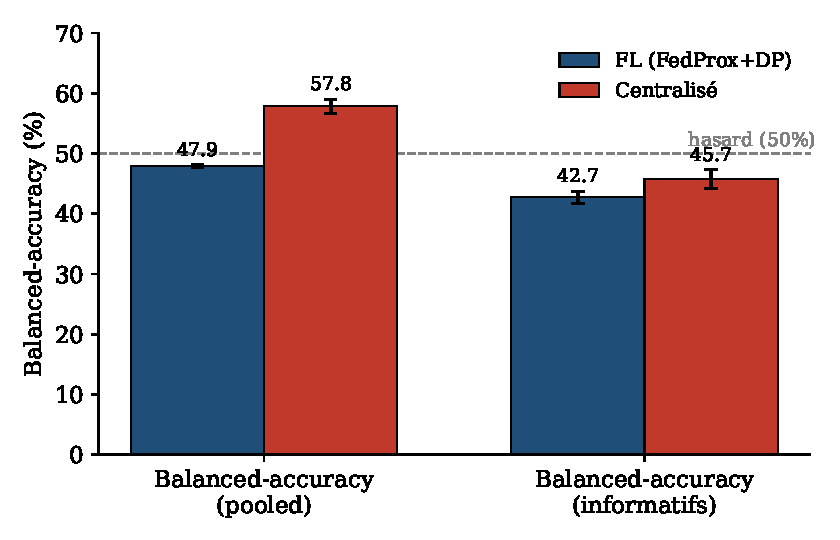
\includegraphics[width=0.75\linewidth]{fig_main_comparison.pdf}
  \caption{Balanced-accuracy, FL vs centralized, pooled metric (15 clients) versus
  metric restricted to the 4 informative clients. The centralized model's apparent
  advantage on the pooled metric shrinks sharply once restricted to genuinely
  informative clients, with both conditions close to chance level.}
  \label{fig:main_comparison}
\end{figure}

\paragraph{Decomposing federation vs privacy.} The comparison above pits
``FL + DP'' against ``centralized without FL or DP'', two conditions that differ
simultaneously along two axes (decentralization and privacy noise), without
isolating them. To determine which of the two explains the measured cost, a third
condition was added: federated FedProx, without DP-SGD (no clipping, no noise),
same learning rate as the FL+DP condition, deliberately not re-tuned so as to
isolate the effect of DP all else being equal (gradient clipping changes the
effective size of the optimization step; not recalibrating the LR genuinely
compares the same optimizer with and without DP, not two different settings).
Result on the same pooled test set, 5 seeds:

\begin{table}[h!]
  \centering
  \caption{Decomposing the cost: centralized (no FL, no DP), FL without DP
  (FedProx alone), FL + DP (average over 5 seeds each, except FL+DP averaged over
  5$\sigma \times$5 seeds).}
  \label{tab:dp_decomposition}
  \begin{tabular}{lccc}
    \toprule
    Metric & Centralized & FL without DP & FL + DP \\
    \midrule
    Accuracy         & $81.95 \pm 0.89\,\%$ & $83.10 \pm 0.92\,\%$ & $82.00 \pm 0.62\,\%$ \\
    Balanced-accuracy (pooled, 15 clients) & $57.84 \pm 1.16\,\%$ & $48.68 \pm 0.73\,\%$ & $47.83 \pm 0.35\,\%$ \\
    \textbf{Balanced-accuracy (4 informative clients)}\textsuperscript{\ddag} & $45.73 \pm 1.54\,\%$ & $45.18 \pm 2.38\,\%$ & $42.73 \pm 0.97\,\%$ \\
    F1 macro (pooled, 15 clients) & $58.56 \pm 1.26\,\%$ & $46.10 \pm 0.75\,\%$ & $45.33 \pm 0.28\,\%$ \\
    \bottomrule
  \end{tabular}

  \vspace{2pt}
  {\footnotesize \textsuperscript{\ddag}See Section~\ref{subsec:dataset}: 11/15
  single-class clients distort the pooled metric.}
\end{table}

On the pooled metric, FL without DP (48.68~\%) and FL + DP (47.83~\%) stay within
less than one point of each other, a gap smaller than their respective standard
deviations. On the 4 informative clients, the gap is more pronounced (45.18~\%
versus 42.73~\%, i.e. 2.45 points): \textbf{DP-SGD noise has a real but secondary
cost}, and this cost is proportionally more visible on the most difficult clients
than on the pooled metric, which dilutes it. In both readings, most of the gap
with the centralized model is already present without any DP-SGD: federation
itself (FedAvg/FedProx aggregation across 15 clients with an extremely
heterogeneous class composition, Section~\ref{subsec:dataset}) dominates the cost
by far, differential privacy adding only a measurable but modest supplement.

Raw accuracy does not distinguish between the three conditions (82.0~\% versus
83.1~\% versus 81.95~\%, within statistical noise). On the pooled metric, the gap
appears clear: the centralized model shows apparent discriminative power
(balanced-accuracy $57.84\,\%$, well above the $50\,\%$ chance level) against an FL
model close to or slightly below chance ($\approx 47.9\,\%$). But on the 4
informative clients (Figure~\ref{fig:main_comparison}), \textbf{the centralized
model collapses too} ($45.73\,\%$, barely above chance), a result discussed in
detail in Section~\ref{subsec:why_cent_wins}, which changes the nature of the
conclusion: it is no longer ``the centralized model solves a problem that FL does
not'', it is ``extreme heterogeneity limits both approaches, with FL adding only a
marginal disadvantage on top'' (see Section~\ref{sec:discussion}).

To put a number on these two readings rather than a visual judgment on mean $\pm$
standard deviation, a Welch test was conducted on the 25 FL checkpoints ($5 \sigma
\times$ 5 seeds) against the 5 centralized checkpoints. The 25 FL checkpoints are
treated as replicates of a single condition, which is defensible since
balanced-accuracy is nearly constant regardless of $\sigma$
(Table~\ref{tab:epsilon_grid_extended}), rather than as 25 independent
measurements of an effect varying with $\sigma$. On raw accuracy, the gap is not
significant ($t=0.11$, $p=0.92$; confirmed by a Mann-Whitney test, $p=0.56$, more
robust to the fragile normality assumption with only 5 values on the centralized
side). On balanced-accuracy, the gap is highly significant ($t=-19.2$, $p < 10^{-4}$;
Mann-Whitney $U=0$, complete separation of the two groups, $p < 10^{-4}$): this is
not a sampling-variance artifact.

\subsection{Privacy vs Utility Trade-off}
\label{subsec:privacy_utility}

Table~\ref{tab:epsilon_grid_extended} details the evolution of the accumulated
privacy budget $\varepsilon$ at round 30, of internal INT8 accuracy (weighted by
client, as a convergence tracking measure), and of balanced-accuracy on the pooled
test set, as a function of the noise multiplier $\sigma$.

\begin{table}[h!]
  \centering
  \caption{Full privacy/utility grid (5 values of $\sigma$, mean
  $\pm$ standard deviation over 5 seeds, $\delta = 10^{-5}$, round 30).}
  \label{tab:epsilon_grid_extended}
  \begin{tabular}{cccc}
    \toprule
    $\sigma$ & $\varepsilon$ (round 30) & INT8 accuracy (internal) & Balanced-acc. (pooled) \\
    \midrule
    0.6 & $5.29 \pm 0.30$ & $81.70 \pm 0.15\,\%$ & $47.87 \pm 0.47\,\%$ \\
    0.8 & $2.18 \pm 0.12$ & $81.60 \pm 0.26\,\%$ & $47.77 \pm 0.26\,\%$ \\
    1.0 & $1.32 \pm 0.13$ & $81.43 \pm 0.46\,\%$ & $47.85 \pm 0.24\,\%$ \\
    1.4 & $0.82 \pm 0.06$ & $81.50 \pm 0.43\,\%$ & $47.67 \pm 0.32\,\%$ \\
    1.8 & $0.54 \pm 0.04$ & $81.60 \pm 0.17\,\%$ & $48.12 \pm 0.38\,\%$ \\
    \bottomrule
  \end{tabular}
\end{table}

\begin{figure}[h!]
  \centering
  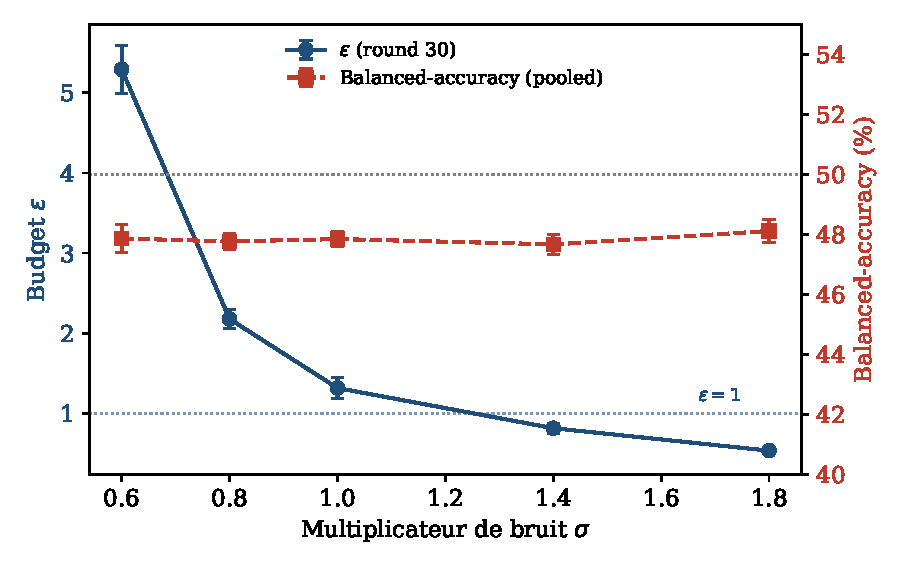
\includegraphics[width=0.8\linewidth]{fig_privacy_utility.pdf}
  \caption{Privacy/utility trade-off: the budget $\varepsilon$ decreases sharply
  with $\sigma$ (left axis) while pooled balanced-accuracy (right axis) remains
  nearly flat across the whole tested range.}
  \label{fig:privacy_utility}
\end{figure}

Epsilon decreases monotonically and smoothly with $\sigma$, exactly as expected
mathematically, which confirms the accountant is functioning correctly. INT8
accuracy and pooled balanced-accuracy remain, meanwhile, nearly constant across
the whole range (Figure~\ref{fig:privacy_utility}): the privacy/utility trade-off
is empirically flat, whether read on the internal metric or on the pooled metric.
The cost measured in Section~\ref{subsec:global_comparison} does not worsen when
stronger privacy is required.

\subsection{Ablation: Impact of Local Personalization}
\label{subsec:ablation_personalization}

Table~\ref{tab:ablation_b} compares, for each value of $\sigma$, the \emph{internal}
accuracy (unweighted average over the 15 clients, measured on their own local test
set) of the global model received from the server (before adaptation) with that
of the same model after that round's local FedProx training epochs.

\begin{table}[h!]
  \centering
  \caption{Local vs global gap (mean $\pm$ standard deviation over 5 seeds),
  internal per-client accuracy, round 30.}
  \label{tab:ablation_b}
  \begin{tabular}{ccc}
    \toprule
    $\sigma$ & Global Model (internal) & Local $-$ global gap \\
    \midrule
    0.6 & $78.08 \pm 1.04\,\%$ & $+0.61 \pm 0.85$ pts \\
    0.8 & $77.64 \pm 0.41\,\%$ & $+0.86 \pm 0.57$ pts \\
    1.0 & $77.75 \pm 0.42\,\%$ & $+0.47 \pm 0.75$ pts \\
    1.4 & $77.48 \pm 0.43\,\%$ & $+0.81 \pm 0.85$ pts \\
    1.8 & $78.13 \pm 0.75\,\%$ & $+0.28 \pm 0.88$ pts \\
    \bottomrule
  \end{tabular}
\end{table}

Local personalization brings here only a marginal and noisy gain (less than 1.2
points on average, sometimes statistically null given the standard deviation).
This result indicates that the added value of FedProx personalization is weak on
this dataset: most of the performance gap plays out between FL and centralized
(Section~\ref{subsec:global_comparison}), not between the global model and the
personalized model within FL.

\subsection{New-Joiner Scenario: Adapting a Pre-trained Model}
\label{subsec:late_joiner}

The personalization gap above is measured on clients who have \emph{already}
participated in FL training. A more realistic, and more demanding, deployment
scenario is that of a nurse who joins the federation \emph{after the fact}: she
receives the global model already trained on the others, without ever having
contributed herself. To simulate this, client 8 (balanced class composition in
both train and test, $36.0\,\%$ stress in test, not single-class, unlike most
other clients, Section~\ref{subsec:dataset}) is fully excluded from federated
training (30 rounds, $\sigma=0.8$, 3 seeds): its contribution is neutralized in
FedProx aggregation (zero weight, \texttt{num-examples}$=0$), so the final global
model has never seen its data. This model is then evaluated directly on client
8's data (``day 1'', zero adaptation), then fine-tuned on its own local training
data (8 epochs, same learning rate as the rest of the pipeline) before
re-evaluation.

\begin{table}[h!]
  \centering
  \caption{New-joiner scenario (client 8, mean $\pm$ standard deviation over 3
  seeds): before and after local adaptation on a model never trained on its data.}
  \label{tab:late_joiner}
  \begin{tabular}{lccc}
    \toprule
    Condition & Accuracy & Balanced-accuracy & Macro F1 \\
    \midrule
    Day 1 (zero adaptation) & $36.56 \pm 0.92\,\%$ & $50.41 \pm 0.72\,\%$ & $27.41 \pm 1.57\,\%$ \\
    After local adaptation (8 epochs) & $51.75 \pm 1.38\,\%$ & $\mathbf{58.51 \pm 1.00\,\%}$ & $\mathbf{51.43 \pm 1.51\,\%}$ \\
    \bottomrule
  \end{tabular}
\end{table}

Without adaptation, the global model is barely at chance level on this new client
(balanced-accuracy $50.41\,\%$): it has never seen its local distribution, and the
extreme Non-IID nature of this dataset (Section~\ref{subsec:dataset}) limits its
direct generalization. After only 8 epochs of local fine-tuning, balanced-accuracy
climbs to $58.51\,\%$ (comparable to the centralized model,
Table~\ref{tab:main_results}) and macro F1 nearly doubles. This is a clearer
result than the ``in-training'' personalization gap of Table~\ref{tab:ablation_b}:
the real value of local adaptation shows up especially for a genuinely new
participant, not for a client already integrated into the training cycle.

\textbf{Important limitation}: this result rests on a single excluded client
(client 8) and 3 seeds, versus 5 seeds everywhere else in this report. This is an
\textbf{illustrative case}, not a result generalizable to all 15 nurses: nothing
guarantees that another excluded client, with a different class composition,
would show an adaptation gain of the same magnitude. A systematic study repeating
this procedure across several clients would be needed for a general conclusion.

\subsection{Per-Class Recall and an Extreme Case: The Most Atypical Client}
\label{subsec:late_joiner_recall}

The balanced-accuracy in Table~\ref{tab:late_joiner} can mask very different error
profiles depending on the class: a model that almost always predicts the same
class can show a balanced-accuracy close to $50\,\%$ without this being a sign of
absence of signal, exactly the trap identified in
Section~\ref{subsec:why_cent_wins}. To check this on the new-joiner scenario, and
push the test to the most unfavorable case, we repeat the same procedure (full
exclusion from training, 30 rounds, $\sigma=0.8$, 3 seeds, 8 epochs of adaptation)
on client 5, one of the 4 informative clients, where a substantial share
($12.7\,\%$) of the global FL+DP model's confident errors is concentrated (full
per-client detail in Section~\ref{subsec:why_cent_wins}).

\begin{table}[h!]
  \centering
  \caption{Per-class recall (default threshold $0.5$), before and after local
  adaptation, min--max range over 3 seeds.}
  \label{tab:late_joiner_recall}
  \begin{tabular}{lcc}
    \toprule
    Client / Condition & Non-stress recall & Stress recall \\
    \midrule
    Client 8, day 1 (zero adapt.)      & $0.00$--$2.48\,\%$   & $99.93$--$100.00\,\%$ \\
    Client 8, after adapt. (8 ep.)      & $32.95$--$37.03\,\%$ & $81.17$--$86.28\,\%$ \\
    \addlinespace
    Client 5, day 1 (zero adapt.)      & $68.00$--$96.00\,\%$ & $0.00$--$1.02\,\%$ \\
    Client 5, after adapt. (8 ep.)      & $100.00\,\%^{\text{a}}$ & $3.13$--$19.66\,\%$ \\
    \bottomrule
  \end{tabular}
  \vspace{2pt}
  {\footnotesize $^{\text{a}}$Exact value, identical across the 3 seeds (25/25
  non-stress windows correctly classified each time), not a rounded range. To be
  taken with caution: client 5's test set has only 25 non-stress windows in total
  (out of 1688), too small a denominator for a reliable recall estimate on this
  single class.}
\end{table}

Per-class recall reveals two symmetric, opposite failures at day 1: client 8's
model predicts almost exclusively ``stress'' (stress recall $\approx 100\,\%$,
non-stress recall $\approx 0\,\%$), while client 5 shows the opposite bias
(non-stress recall $68$--$96\,\%$, stress recall $\leq 1.02\,\%$), consistent with
the AUC close to or below $0.5$ already measured for this client. In both cases,
the day-1 balanced-accuracy close to $50\,\%$ was hiding a strong systematic bias,
not an absence of signal.

Local adaptation partially corrects both biases in the opposite direction, but
incompletely for client 5: at an unchanged threshold ($0.5$), stress recall only
rises to $3.13$--$19.66\,\%$ (mean $12.15\,\%$). The model continues to miss the
vast majority of real stress episodes on this client, which would be clinically
unacceptable for an alert system. Client 8, conversely, reaches a stress recall of
$81.17$--$86.28\,\%$ after adaptation, a much more usable profile.

\paragraph{Complementary diagnostic (not a deployment protocol): post-adaptation
threshold calibration.} The same threshold sweep as Section~\ref{subsec:why_cent_wins}
applied to the adapted models reveals, for both clients, additional recall
potential left unexploited at the default threshold, but in opposite directions:
the optimal threshold drops to $0.001$ for client 5 (stress recall raised to
$26.46$--$66.63\,\%$, mean $42.53\,\%$) and rises to $0.950$ for client 8 (stress
recall reduced to $71.93$--$75.98\,\%$ in favor of non-stress recall, raised to
$59.05$--$59.65\,\%$). \textbf{This sweep selects the threshold that maximizes the
metric on the test set later used to report it: it is a legitimate diagnostic
tool for revealing a calibration problem, not a validated deployment protocol}.
The resulting recall figure is an optimistic upper bound, not a performance
expected in production. Note further that client 5's optimal threshold hits the
lower bound of the sweep ($0.001$), the same boundary artifact already
encountered in Section~\ref{subsec:why_cent_wins}: the exact value therefore
remains provisional and is not reported as a final result. The direction of
divergence between the two clients (toward $0$ for one, toward $1$ for the other)
is nonetheless consistent with their opposite day-1 biases, and \emph{suggests}
that a per-client calibrated threshold (on a dedicated validation split, distinct
from the test set, never done in this work) could bring a real deployment gain.
With only $N=2$ clients tested, this remains a lead to verify, not an established
conclusion.

\textbf{Limitations}: these results rest on two excluded clients (8 and 5) and 3
seeds each, versus 5 seeds everywhere else in this report. These are
\textbf{illustrative cases}, not a result generalizable to the 15 nurses.

\subsection{The Same Scenario Under FedPer: A New Joiner With No Head History}
\label{subsec:fedper_late_joiner}

The new-joiner scenario is replayed under FedPer (Section~\ref{subsec:fedper}) on
the same two clients (8 and 5, full exclusion from training, 30 rounds,
$\sigma=0.8$, 3 seeds). \textbf{The definition of ``day 1'' necessarily differs
between the two architectures, and this is not an artifact to correct but a
direct consequence of their design}: under FedProx
(Section~\ref{subsec:late_joiner}), the new joiner inherits a head that is
\emph{poorly calibrated but informed} (that of the final global model); under
FedPer, there is literally \textbf{no head to inherit} (\texttt{fc3} is never
transmitted), so FedPer's ``day 1'' is evaluated with a \emph{blank, randomly
initialized} head, placed on the shared extractor (never trained on this
client's data). These are not two measurements of the same phenomenon all else
being equal: they should not be read as directly comparable term for term.

\begin{table}[h!]
  \centering
  \caption{FedPer, new-joiner scenario: day 1 (blank random head) vs after
  onboarding (training \texttt{fc3} only, frozen extractor, 8 epochs), min--max
  range over 3 seeds.}
  \label{tab:fedper_late_joiner}
  \begin{tabular}{lcc}
    \toprule
    Client / Condition & Balanced-accuracy & Recall (non-stress~/~stress) \\
    \midrule
    Client 8, day 1 (blank head)   & $50.06$--$69.66\,\%$ & $0.12$--$93.76\,\%$~/~$40.58$--$100.00\,\%$ \\
    Client 8, after onboarding       & $54.80$--$69.57\,\%$ & $62.37$--$80.86\,\%$~/~$43.14$--$58.28\,\%$ \\
    \addlinespace
    Client 5, day 1 (blank head)   & $5.31$--$50.00\,\%$  & $4.00$--$100.00\,\%$~/~$0.00$--$6.61\,\%$ \\
    Client 5, after onboarding       & $73.33$--$80.41\,\%$ & $96.00$--$100.00\,\%$~/~$46.66$--$64.82\,\%$ \\
    \bottomrule
  \end{tabular}
\end{table}

\paragraph{An additional source of variance, distinct from the one already
documented.} FedPer's day 1 shows considerable dispersion across seeds (client 8:
balanced-accuracy 50.1~\% to 69.7~\%; client 5: 5.3~\% to 50.0~\%), markedly wider
than FedProx's day 1 (deterministic for a given checkpoint). This variance has an
identified cause, distinct from the temporal drift already documented for client
5 (Section~\ref{subsec:why_cent_wins}): it comes solely from the random
initialization of the blank head, a noise source that does not exist under
FedProx where the inherited head is deterministic for a given final model. For
client 5, two of the three head-initialization seeds collapse toward an almost
constant ``non-stress'' prediction (balanced-accuracy exactly 50~\%, stress
recall 0~\%) while the third produces a result worse than chance on both classes
simultaneously ($5.3\,\%$). These two failures have different mechanisms (an
untrained classifier, not a failing extractor): they should not be confused with
a signal of poor extractor quality.

\paragraph{After onboarding: a net gain, and above all markedly more stable.}
Training only \texttt{fc3} for 8 epochs (frozen extractor) sharply narrows the
dispersion and improves client 5's stress recall at the default threshold
($0.5$, with no threshold recalibration at all): $46.66$--$64.82\,\%$ (mean
$57.19\,\%$), versus $3.13$--$19.66\,\%$ (mean $12.15\,\%$) for FedProx's full
post-hoc adaptation at the same default threshold
(Table~\ref{tab:late_joiner_recall}), and even comparable to FedProx's
threshold-calibration diagnostic (not deployable as is,
Section~\ref{subsec:why_cent_wins}), obtained here \emph{without} any threshold
being touched. Client 8 shows a narrowing of dispersion rather than a net gain
(comparable mean balanced-accuracy, standard deviation divided by more than 2):
FedPer onboarding mainly stabilizes the result; the effect is less dramatic than
for client 5 but in the same direction.

\textbf{Limitations}: the same caveats as for the FedProx scenario (N=2 clients,
3 seeds, illustrative case), with here an additional caveat specific to FedPer:
since day-1 variance depends on the head's random initialization, a different
initialization seed could produce a substantially different day 1, independent of
the data-partition seed.

\subsection{Quantization and Weight Dynamic Range}

The dynamic range of the weights (defined as $\max(|w|) - \min(|w|)$) was measured
on the final model after 30 rounds of training. Figure~\ref{fig:dynamic_range}
presents this measure over the whole network (global dynamic range) as well as on
the first linear layer (\texttt{fc1.weight}).

\begin{figure}[h!]
  \centering
  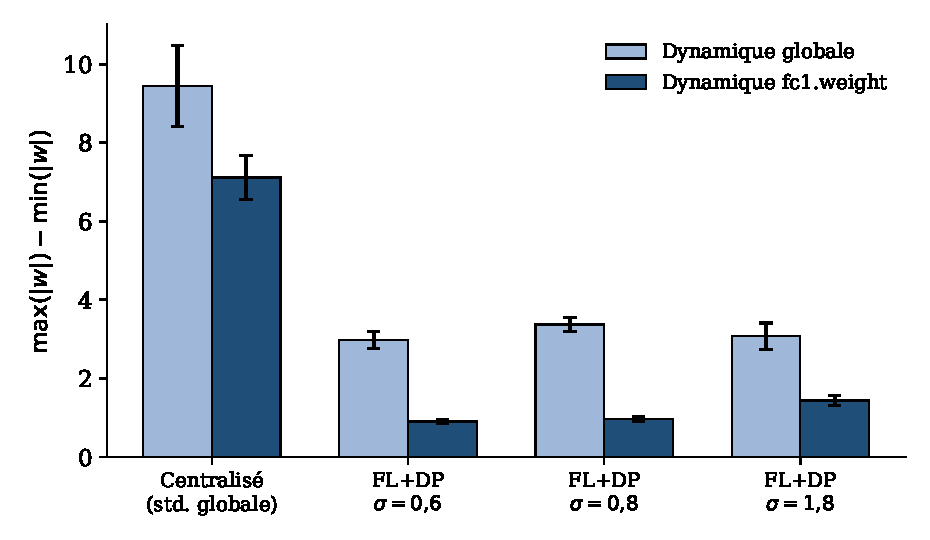
\includegraphics[width=0.8\linewidth]{fig_dynamic_range.pdf}
  \caption{Dynamic range of the weights (mean $\pm$ standard deviation over 5
  seeds) by training mode and DP noise level.}
  \label{fig:dynamic_range}
\end{figure}

\subsection{Memory Footprint (Peak RAM)}

Peak RAM usage was measured dynamically on a client at round 30, immediately
before and during Opacus's call to \texttt{get\_epsilon()}.

\begin{table}[h!]
  \centering
  \caption{Peak RAM consumption (MB, mean $\pm$ standard deviation over 5 seeds)
  at round 30, before and during the privacy computation, as a function of
  $\sigma$.}
  \label{tab:ram_results}
  \begin{tabular}{cccc}
    \toprule
    $\sigma$ & Noise level & Before \texttt{get\_epsilon()} & During \texttt{get\_epsilon()} \\
    \midrule
    0.6 & Low    & $0.18 \pm 0.00$~MB & $33.65 \pm 3.30$~MB \\
    0.8 & Moderate-low & $0.18 \pm 0.00$~MB & $20.48 \pm 1.50$~MB \\
    1.0 & Moderate    & $0.18 \pm 0.00$~MB & $16.05 \pm 1.70$~MB \\
    1.4 & High      & $0.18 \pm 0.00$~MB & $13.44 \pm 1.00$~MB \\
    1.8 & Very high & $0.37 \pm 0.42$~MB$^{*}$ & $11.34 \pm 0.43$~MB \\
    \bottomrule
  \end{tabular}

  \vspace{2pt}
  {\footnotesize $^{*}$4 of the 5 seeds give $\approx 0.18$~MB, consistent with
  the other rows; a single seed produces an isolated value of $1.11$~MB, pulling
  the average up. Most likely a one-off measurement artifact
  (\texttt{tracemalloc} / Python garbage collector pass) rather than a real
  effect of $\sigma$, otherwise the same increase would be observed on the other
  seeds.}
\end{table}

\section{Interpretation and Discussion}
\label{sec:discussion}

This section offers a theoretical and methodological analysis of the observed
phenomena.

\subsection{What the FL/Centralized Gap Really Reveals: A Shared Limitation, Not
a Centralized Advantage}
\label{subsec:why_cent_wins}

On the pooled test set (15 clients), the centralized model shows an apparent
advantage in balanced-accuracy (57.84~\% versus $\approx$ 47.9~\% for FL,
Section~\ref{subsec:global_comparison}). \textbf{This reading does not survive
per-client inspection.} 11 of the 15 clients have a single-class test set
(Section~\ref{subsec:dataset}) where any constant prediction mechanically
achieves $100\,\%$: they dominate the pooled metric and mask what actually
happens on the 4 clients (4, 5, 8, 12) whose test set is genuinely mixed, the
only ones on which balanced-accuracy is a meaningful measure of the model's
discriminative power.

\paragraph{On the informative clients, the centralized model collapses too.}
Restricted to these 4 clients, the centralized model's balanced-accuracy drops to
$45.73 \pm 1.54\,\%$, barely above chance, and its AUC-ROC to $0.2669 \pm
0.0197$. \textbf{Caution about this sample size}: this pooled AUC rests on only 4
clients, a restricted sample of the same order of magnitude as one for which this
document already applies an explicit caveat (client 5's 25 non-stress windows
alone, Table~\ref{tab:late_joiner_recall}). Part of the gap from $0.5$ could stem
from sampling noise rather than from a systematically inverted learned
relationship, even though the sign consistency with the per-client diagnostic
below makes this reading unlikely. By the same logic already established for
client 5's diagnostic further in this section:
\textbf{an AUC significantly below $0.5$ does not signal an absence of signal,
but a partially \emph{inverted} ranking}: the probabilities predicted by the
centralized model rank test windows in the opposite direction from ground truth
more often than a random ranking would. The centralized model has therefore not
simply ``learned nothing'' on these clients; it has learned a partially wrong
relationship. The decision-threshold sweep (from $10^{-3}$ to $0.99$, on the
already-produced probabilities, no retraining) confirms this indirectly: the
centralized model's optimal threshold collapses onto $0.001$ (predicting
``stress'' almost systematically, i.e. inverting the default prediction rather
than calibrating it), plateauing at \emph{exactly} $50.00 \pm 0.00\,\%$: a
threshold correction that compensates for the inversion without resolving it,
identical in form to what this document had so far attributed to FL alone. FL+DP,
on these same 4 clients, shows the same signature, slightly more pronounced
(balanced-accuracy $42.73 \pm 0.97\,\%$, AUC $0.2047 \pm 0.0232$, best threshold
also $0.001$, plateau at $46.98 \pm 1.28\,\%$, not even reaching the theoretical
floor, a sign that the inversion is less fully compensable there by threshold
choice alone). \textbf{The central message of this document changes
accordingly}: it is not a matter of ``why the centralized model solves a problem
that FL does not'', but of ``why neither architecture learns a reliable
relationship on the most atypical clients''. The actual gap between the two (3
to 5 points of balanced-accuracy depending on the metric) is a marginal
disadvantage of FL on top of an underlying problem common to both, not proof
that FL is structurally unsuitable.

\paragraph{Statistical significance of the centralized-vs-FL gap, on the
informative clients.} A Welch test and a Mann-Whitney test were conducted on the
balanced-accuracy of the 4 informative clients: centralized (5 seeds) versus
FL+DP (25 values, $5\sigma \times$ 5 seeds), and centralized versus FL without DP
(5 seeds). Result, consistent with the decomposition that follows:
\textbf{centralized vs FL+DP is statistically significant} (Welch $t=4.21$,
$p=9.8\times10^{-3}$; Mann-Whitney $U=123/125$, $p=5.6\times10^{-5}$), but
\textbf{centralized vs FL without DP is not} (Welch $t=0.44$, $p=0.68$;
Mann-Whitney $U=15/25$, $p=0.69$). On these specific clients, federation alone
(without privacy) is not statistically distinguishable from the centralized
model, and it is the addition of DP-SGD noise that creates the measurable gap
with the centralized model. This is a nuance relative to the pooled metric, where
most of the gap was attributed to decentralization rather than to privacy,
consistent with the already-established observation that the cost of DP noise is
proportionally more visible on the difficult clients than on the pooled metric.

\textbf{Verification that this contrast (significant versus non-significant)
does not simply reflect a statistical-power imbalance} between the two
comparisons (FL+DP: $n=25$ versus FL without DP: $n=5$, the same size as the
centralized model), a classic pitfall already debunked elsewhere in this document
(Section~\ref{subsec:duration_vs_granularity}). Two independent checks:
(1)~effect size (Cohen's $d$), insensitive to this imbalance, remains far
greater for centralized vs FL+DP ($d=2.81$, large effect) than for centralized vs
FL without DP ($d=0.28$, small effect), a factor of 10 between the two effect
sizes, not just between the two $p$-values; (2)~repeated subsampling of FL+DP
down to $n=5$ (2,000 draws without replacement, to exactly match the power of the
centralized-vs-FL-without-DP test) remains significant at $p<0.05$ in $99.7\,\%$
of draws (median $p =9.2\times10^{-3}$, nearly identical to the
$p=9.8\times10^{-3}$ on the full sample). The observed contrast is therefore not
a sample-size artifact: at equal power, the centralized/FL+DP gap is almost
always detected, unlike the centralized/FL-without-DP gap.

\textbf{A limitation not to be glossed over regarding the scope of this
significance.} The 25 (or 5) tested values come from 5 training seeds and 5
values of $\sigma$, sources of training noise, not clinical diversity. The
measured significance demonstrates that the gap is \emph{reproducible across
seeds and noise levels, on these 4 specific clients}; it does not demonstrate
that the phenomenon would generalize to a 5\textsuperscript{th} client profile
with a mixed test set, since this dataset provides no other one to check this
against. This is a structural characteristic of this dataset (only 4 clients
with a genuinely mixed test set, Section~\ref{subsec:dataset}), not a weakness of
the statistical method used, but it strictly bounds the scope of the conclusion:
a result solid on \emph{these} 4 nurses, not yet a demonstrated generalization to
any heterogeneous patient population.

\paragraph{Decomposing federation vs privacy, on both metrics.}
Table~\ref{tab:dp_decomposition} isolates the contribution of DP-SGD noise:
\begin{itemize}
  \item \textbf{On the pooled metric}, FL without DP (48.68~\%) and FL + DP
  (47.83~\%) are within less than one point of each other: DP-SGD noise appears
  nearly free there.
  \item \textbf{On the 4 informative clients}, the gap is more pronounced (FL
  without DP $45.18 \pm 2.38\,\%$ versus FL+DP $42.73 \pm 0.97\,\%$, i.e. 2.45
  points): the cost of privacy noise is real, simply diluted by the pooled
  metric, which drowns it under the trivial clients. It nonetheless remains
  secondary compared to the gap with the centralized model, which persists
  almost identically with or without DP-SGD.
\end{itemize}
In both readings, FedAvg/FedProx aggregation across 15 clients this
heterogeneous (Section~\ref{subsec:dataset}) dominates the measured cost;
differential privacy adds a measurable but, contrary to what the pooled metric
suggests, clearly secondary supplement.

\paragraph{Concentration of errors, revisited.} A per-client inspection of
windows where the FL+DP model is confidently wrong (predicted probability
$>0.9$ for the predicted class), aggregated over the 25 grid checkpoints, shows
that client 3 alone concentrates $31.1\,\%$ of all such errors, the top
contributor across all 25 checkpoints without exception, followed by the 4
informative clients (client 12: $29.3\,\%$, client 8: $19.4\,\%$, client 5:
$12.7\,\%$, client 4: $6.3\,\%$); together, these five clients account for
$98.9\,\%$ of confident errors, the other 10 single-class clients collectively
representing only about $1\,\%$. The mechanism differs by case: on the 4
informative clients, it is a signal genuinely difficult to learn (previous
paragraphs); on client 3, it is the same majority-class bias already noted in
Section~\ref{subsec:dataset}, this time working against it (its only present
test class is the global minority class), a more mechanical phenomenon than the
4 informative clients but one that nonetheless confirms the central finding: the
FL+DP model's errors concentrate almost exclusively on clients where there is
genuinely something non-trivial to get right or wrong (whether a difficult
signal or a reversed class bias), not on the 10 single-class clients aligned
with the majority bias. This finding is part of a broader problem also affecting
the centralized model, not a pathology specific to FL.

\paragraph{A mitigation tested: class-weighted loss.} Since per-client class
imbalance (Section~\ref{subsec:dataset}) appears central to the problem, a
natural lead is to weight the local loss function by the inverse of the global
class frequency (computed once on the aggregate of all clients' training
partitions). Targeted check at $\sigma=0.8$ (5 seeds, not the whole grid):

\begin{center}
\begin{tabular}{lccc}
  \toprule
  Condition ($\sigma=0.8$) & Accuracy & Balanced-accuracy & Macro F1 \\
  \midrule
  Standard FL + DP        & $81.84 \pm 0.49\,\%$ & $47.77 \pm 0.29\,\%$ & $45.33 \pm 0.19\,\%$ \\
  FL + DP + weighted loss & $81.73 \pm 0.65\,\%$ & $47.66 \pm 0.40\,\%$ & $45.21 \pm 0.25\,\%$ \\
  \bottomrule
\end{tabular}
\end{center}

An honest, negative result: the gap (0.11 point of balanced-accuracy) is within
noise; weighted loss brings no measurable gain here. This is consistent with the
decomposition above: reweighting each client's \emph{local} loss cannot correct
an effect that emerges from \emph{aggregation} across 15 updates this
heterogeneous (including several single-class clients,
Section~\ref{subsec:dataset}): the problem does not lie at the level of the
individual loss function. Leads acting directly on aggregation (reweighting each
client's contribution to the FedProx average, or a stronger personalization
architecture) seem more promising and remain to be explored.

This work therefore does not so much quantify ``the price of privacy and
decentralization'' as \textbf{the difficulty, common to every architecture, of
generalizing over a nurse population this heterogeneous}: even the centralized
model, which suffers none of FL's constraints, fails on the most atypical
clients (balanced-accuracy barely above chance, AUC below it). FL's additional
disadvantage relative to the centralized model (3 to 5 points depending on the
metric) remains real, measurable, and non-negligible, but it is a supplement to
an underlying problem, not the problem itself. This distinction matters for
interpretation: since the centralized model is in any case not a genuinely
available alternative for this use case (aggregating the raw physiological
signals of 15 nurses on a single server would constitute a health-data
processing activity hardly compatible with the GDPR's data-minimization
principle, Art.~5~\cite{gdpr2016}, as noted in the introduction), FL remains the
only viable approach in practice, and this work shows that it adds only a
marginal cost on top of a limitation that the centralized model would not solve
either. The most promising future work (more informative features,
personalization architectures such as FedPer and FedRep+SCAFFOLD below) is
therefore aimed less at ``catching up with the centralized model'' than at
reducing the effect of Non-IID heterogeneity itself, a problem that goes beyond
the FL-versus-centralized choice.

\subsection{An Architecture Tested for Stronger Personalization: FedPer}
\label{subsec:fedper}

The ``stronger personalization'' lead mentioned above was tested directly, via
\textbf{FedPer}~\cite{arivazhagan2019federated}: the feature extractor
(\texttt{fc1}, \texttt{fc2}) remains globally aggregated as in FedProx, but the
final classification layer (\texttt{fc3}) is \emph{never} transmitted to the
server or aggregated: it stays local to each client, trained continuously on its
own data throughout the 30 rounds. Unlike Ditto (two full networks per client,
regularized toward each other by a proximal term), FedPer modifies only a single
network and requires only a filter on the keys of the transmitted weight
dictionary, an implementation difference that proved relevant: this repository's
history contains a documented synchronization bug on the Ditto branches
(\texttt{f2d0b15}, \texttt{a3d8107}, \texttt{6e6ee40}, local weights mistakenly
overwritten with global weights at every round), a class of error that
structurally does not exist with FedPer since there is nothing to resynchronize.

\paragraph{Evaluation methodology: a difference to state explicitly.} Unlike
FedProx (Section~\ref{subsec:global_comparison}), FedPer produces \textbf{no
single evaluable global model}: the final server checkpoint contains only the
extractor (\texttt{fc1}, \texttt{fc2}), never a classification head. Each test
window is therefore scored by the model belonging to the client it comes from
(shared extractor + that client's local head), and predictions from all clients
are then pooled to obtain global metrics. This choice is not a workaround: it is
the only evaluation consistent with the architecture, and it is in fact
\textbf{more representative of a real deployment} than FedProx's single model,
since each wearable would run its own model anyway.

\begin{table}[h!]
  \centering
  \caption{FedPer vs FedProx+DP (evaluation methodology specific to each
  architecture, see text), average over 5$\sigma\times$5 seeds (n=25 each).}
  \label{tab:fedper_comparison}
  \begin{tabular}{lcc}
    \toprule
    Metric & FedProx + DP & FedPer \\
    \midrule
    Accuracy (pooled, 15 clients)      & $82.02 \pm 0.62\,\%$ & $82.97 \pm 2.07\,\%$ \\
    Balanced-accuracy (pooled, 15 clients) & $47.86 \pm 0.35\,\%$ & $65.06 \pm 2.72\,\%$ \\
    \textbf{Balanced-accuracy (4 informative clients)}\textsuperscript{\ddag} & $42.73 \pm 0.97\,\%$ & $\mathbf{48.44 \pm 3.65\,\%}$ \\
    \textbf{AUC-ROC (4 informative clients)}\textsuperscript{\ddag} & $0.2047 \pm 0.0232$ & $\mathbf{0.4417 \pm 0.1022}$ \\
    Communication (FIT, average) & $5.320$~KB          & $5.188$~KB ($-2.5\,\%$) \\
    \bottomrule
  \end{tabular}

  \vspace{2pt}
  {\footnotesize \textsuperscript{\ddag}Metric restricted to clients with a
  genuinely mixed test set (Section~\ref{subsec:dataset}), the most clinically
  honest measure.}
\end{table}

On the pooled metric, the gap is very pronounced (Welch $t=30.69$,
$p=3.1\times10^{-21}$; Mann-Whitney $U=625/625$, complete separation), but this
figure is inflated by the 11 single-class clients (Section~\ref{subsec:dataset}),
on which both architectures obtain very close, often identical, scores.
\textbf{On the 4 informative clients, the actual gap is more modest but remains
statistically solid} (Welch $t=7.56$, $p=3.6\times10^{-8}$; Mann-Whitney
$U=590/625$, $p=7.7\times10^{-8}$): +5.7 points of balanced-accuracy in favor of
FedPer, with a markedly higher variance than on the pooled metric (standard
deviation $3.65\,\%$ versus $2.14\,\%$). FedPer helps on the difficult clients,
but less spectacularly, and less uniformly, than the pooled metric suggests. Full
detail (results per $\sigma$ and per seed, statistical tests on both metrics) is
kept in \texttt{resultsfeat/fedper\_results\_summary.md}, separately from this
document.

\paragraph{Interpretation: a direct confirmation, but of more modest magnitude
than it appears.} This result complements the FL-versus-DP decomposition above,
which had attributed the balanced-accuracy cost to \emph{aggregation}, not to
privacy noise. FedPer tests this hypothesis directly by removing aggregation of
the single layer responsible for the final decision, and part of the cost
disappears, on the metric that matters clinically. The gap measured on the
informative clients (also verified by ruling out an accidental checkpoint mix-up
between the two conditions) should not come as a surprise, but \textbf{should
also not be attributed to a single factor}: FedPer and FedProx differ here
simultaneously along \emph{two axes}: (1)~the \textbf{duration} of
personalization (30 continuous rounds during training, versus 8 epochs of
post-hoc fine-tuning for FedProx, Table~\ref{tab:ablation_b}) and (2)~the
\textbf{granularity} (only the classification head for FedPer, versus the entire
network for FedProx's post-hoc fine-tuning). \textbf{These two factors have since
been isolated separately} (Section~\ref{subsec:duration_vs_granularity}, starting
from the same initial checkpoint and with re-seeded fine-tuning for a paired
statistical test over 5 seeds): \emph{granularity} dominates by far (+6.5 to +7.4
points of balanced-accuracy, $p<0.03$). Personalizing only the head, from the
same extractor, clearly outperforms fine-tuning the entire network, likely by
limiting overfitting on the small amount of local data available per client, and
\emph{duration} also matters, but far more modestly (+1 to +2 points, $p<0.02$).
Raw accuracy also improves, but marginally and only barely significantly
($+0.95$ point, $p=4.0\times10^{-2}$): FedPer therefore does not trade raw
accuracy for balanced recall, but this joint gain on accuracy is tenuous, unlike
the net and highly significant gain observed on balanced-accuracy and AUC.

\subsection{Duration or Granularity? Granularity Dominates, Duration Matters a
Little}
\label{subsec:duration_vs_granularity}

To settle which of the two factors above dominates, FedProx+DP ($\sigma=0.8$,
final checkpoint) is fine-tuned offline on the local training data of each of the
4 informative clients, starting from the \textbf{same} checkpoint in every
condition and varying only one factor at a time: duration (8 versus 30 epochs)
and granularity (entire network unfrozen versus only the \texttt{fc3} head
unfrozen). A first test directly compared full fine-tuning to FedPer (Tier 1):
this comparison confounded granularity with the fact that FedPer starts from
\emph{its own} extractor, trained under an entirely different aggregation regime
(30 rounds with no proximal term, never influenced by an aggregated
\texttt{fc3}). This is corrected below by systematically starting from the same
starting point. Fine-tuning is explicitly re-seeded for each seed to allow a
rigorous paired statistical test (5 values per condition, as everywhere else in
this document).

\begin{figure}[h!]
  \centering
  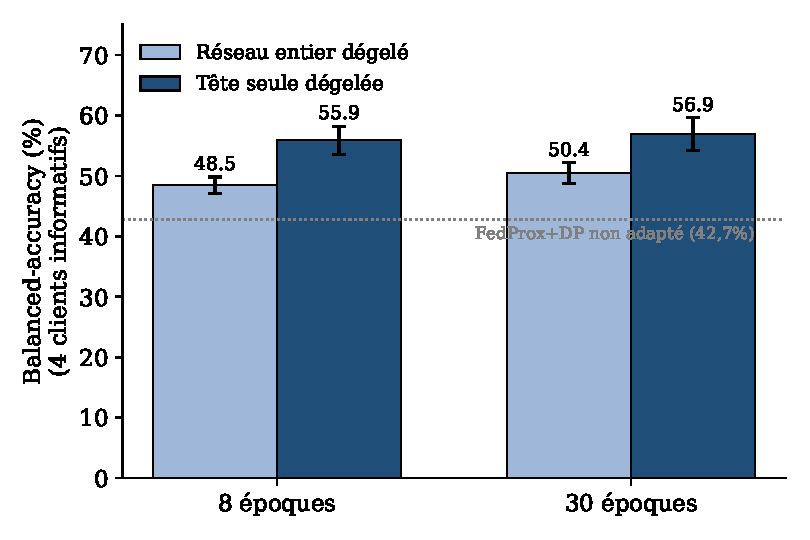
\includegraphics[width=0.7\linewidth]{fig_duration_granularity.pdf}
  \caption{Balanced-accuracy on the 4 informative clients, entire network
  unfrozen versus head only unfrozen, at 8 and 30 epochs, starting from the same
  initial checkpoint. The dashed line marks the unadapted FedProx+DP level.}
  \label{fig:duration_granularity}
\end{figure}
{\footnotesize Balanced-accuracy (mean $\pm$ standard deviation, 5 seeds), pooled
over the 4 informative clients. Reference: unadapted FedProx+DP $42.73 \pm
0.97\,\%$; FedPer (its own extractor, 30 continuous rounds) $48.44 \pm
3.65\,\%$.}

Based on Figure~\ref{fig:duration_granularity}, a paired $t$-test (5 seeds, each
seed compared to itself across conditions) quantifies the two effects:
\textbf{granularity dominates by far} ($+7.39$ points at 8 epochs, $t=5.26$,
$p=6.2\times10^{-3}$; $+6.51$ points at 30 epochs, $t=3.64$,
$p=2.2\times10^{-2}$), \textbf{but duration also matters, modestly} ($+1.94$
point for the entire network, $t=8.11$, $p=1.3\times10^{-3}$; $+1.05$ point for
the head alone, $t=4.43$, $p=1.2\times10^{-2}$). \textbf{This is a revision of an
earlier, non-seeded test that had wrongly concluded that duration had no
effect}: the lack of control over shuffling-order noise was masking a real but
small effect, consistent in sign across the 5 seeds once this noise was
controlled. The paired Wilcoxon test, additionally, plateaus at $p=0.0625$ in all
four cases, a floor artifact specific to $n=5$ pairs whose differences all share
the same sign (the minimum $p$ attainable with so few seeds), not a sign of
doubtful significance; the $t$-test remains the appropriate read here.

\textbf{Correction for multiple comparisons.} Four paired $t$-tests are conducted
on this same set of results; a Bonferroni correction ($\alpha = 0.05/4 = 0.0125$)
is therefore applied as a precaution. \textbf{Both duration effects and
granularity at 8 epochs remain significant after correction} (duration, entire
network, $p=1.3\times10^{-3}$; duration, head only, $p=1.2\times10^{-2}$;
granularity, 8 epochs, $p=6.2\times10^{-3}$, an order of magnitude below the
adjusted threshold); \textbf{only granularity at 30 epochs no longer survives the
corrected threshold} ($p=2.2\times10^{-2}$). This is consistent with the rest of
the section rather than an isolated anomaly: at 30 epochs, the entire network has
had more time to close part of its gap thanks to the duration effect
demonstrated above, which mechanically narrows the gap between the two
granularities and statistically weakens precisely this comparison. The main
message is not weakened by this: it is the less central of the two comparisons
(the one where the gap already narrows), not the one carrying the conclusion.

\textbf{At equal granularity, personalizing longer helps a little; at equal
duration, personalizing only the head helps far more.} The head alone likely
limits overfitting on the small amount of local data available per client (34
parameters adjusted versus 1,362 for the entire network), a plausible
explanation, consistent with common fine-tuning-on-small-target-domain practice,
but not verified further here.

This result revises the reading of Section~\ref{subsec:fedper}: FedPer's
advantage comes both from the fact that personalization occurs and, to a much
lesser extent, from its continuous duration, but above all from its
\emph{granularity} (head only), the dominant factor, a design choice that proves
relevant rather than a mere implementation detail.

\paragraph{A limitation not to be glossed over.} The absence of a single global
model has a deployment cost: there is no universal firmware to distribute to all
nurses. Each wearable must receive (and update) its own classification head in
addition to the shared extractor, which slightly complicates deployment
logistics compared to FedProx. The measured communication gain ($-2.5\,\%$) is
real but mechanically modest on an architecture already this tiny (1,362
parameters): the head weighs only 34 parameters out of that total.

\subsection{Exploring the Best Possible Architecture Outside the TinyML
Constraint}
\label{subsec:fedrep_scaffold}

\textbf{This subsection deliberately relaxes the TinyML constraint} (microcontroller
footprint, firmware size) to explore the best architecture attainable under
\emph{security-only} constraints (no raw data centralized, formal DP guarantee on
what is transmitted). It is not comparable to the previous sections in terms of
embedded-deployment objective, and does not replace the deployable MLP Tiny
architecture, which remains this work's main contribution.

\paragraph{Architecture.} Three elements distinguish this architecture from
FedPer: (1)~a \textbf{two-layer classification head} (16$\to$16$\to$2, 306
parameters) instead of a single linear layer (34 parameters), still never
transmitted or aggregated; (2)~\textbf{DP-SGD restricted to the shared
extractor}: Opacus's clipping and Gaussian noise apply only to the parameters
actually transmitted to the server, the head being trained without noise;
(3)~\textbf{SCAFFOLD}~\cite{karimireddy2020scaffold} replaces FedProx's proximal
term as the Non-IID drift-correction mechanism on the shared extractor: each
client maintains a control variable $c_i$, transmitted to the server under a
dedicated prefixed key to benefit from native aggregation, with client-side
rescaling ensuring that the partition-size-weighted average (standard for model
weights) correctly reconstructs the simple unweighted average that SCAFFOLD
requires for $c_{\text{global}}$.

\textbf{Two factors change simultaneously relative to FedPer, not disentangled in
this work}: head capacity (1 layer versus 2) and the drift-correction mechanism
(FedProx versus SCAFFOLD). A result better than FedPer does not tell us which of
the two dominates, absent a further ablation not performed here: the same
methodological limitation already noted between FedPer and FedProx
(Section~\ref{subsec:fedper}).

\paragraph{A numerical incident fixed along the way, documented for
transparency.} The first pass of the grid diverged (NaN): the SCAFFOLD
correction, applied after DP-SGD clipping, was itself never bounded, whereas the
actual gradient is (at $\text{max\_grad\_norm}$). With $c_i$ accumulating round
after round, the correction eventually dominated the protected gradient, a
feedback loop that made the weights explode within a few rounds. This is fixed by
bounding the correction's norm to the same scale as the DP clipping before adding
it to the gradient, validated on an extended sweep (12 rounds, not just the 3
rounds of the initial quick test) before replaying the full grid: 25/25 runs, no
NaN, no failure.

\paragraph{Methodological discovery: domination by single-class clients.} While
digging into a seemingly remarkably stable balanced-accuracy result (nearly
identical to two decimal places across several seeds), per-client inspection
revealed that \textbf{11 of the 15 clients have a single-class test set} (only
one class present, deterministic split hence identical for any seed,
Section~\ref{subsec:dataset}): a constant prediction mechanically achieves
$100\,\%$ there, regardless of actual model quality. These 11 clients dominate
balanced-accuracy pooled over the 15 clients, masking actual performance on the 4
clients with a genuinely mixed test set (clients 4, 5, 8, 12). \textbf{This
limitation applies retroactively to every pooled 15-client metric reported
earlier in this document} (Tables~\ref{tab:main_results},
\ref{tab:dp_decomposition}, \ref{tab:fedper_comparison}), explicitly flagged in
the synthesis (Section~\ref{subsec:synthesis_limits}) rather than left implicit.
A second metric, restricted to the 4 informative clients, is therefore computed
in addition for all three architectures.

\begin{table}[h!]
  \centering
  \caption{Comparison of FedProx+DP / FedPer / FedRep+SCAFFOLD (average over
  5$\sigma\times$5 seeds, n=25 each), pooled over 15 clients versus restricted to
  the 4 clients with a genuinely mixed test set.}
  \label{tab:fedrep_scaffold_comparison}
  \begin{tabular}{lcccc}
    \toprule
    Balanced-accuracy & FedProx+DP & FedPer & FedRep+SCAFFOLD \\
    \midrule
    Pooled (15 clients)            & $47.86 \pm 0.35\,\%$ & $65.06 \pm 2.78\,\%$ & $\mathbf{77.57 \pm 0.72\,\%}$ \\
    Informative clients (4/15)     & $42.73 \pm 0.97\,\%$ & $48.44 \pm 3.65\,\%$ & $\mathbf{59.89 \pm 0.22\,\%}$ \\
    AUC-ROC (informative clients)  & $0.2047 \pm 0.0232$  & $0.4417 \pm 0.1022$  & $\mathbf{0.7269 \pm 0.0035}$ \\
    \bottomrule
  \end{tabular}
\end{table}

\begin{figure}[h!]
  \centering
  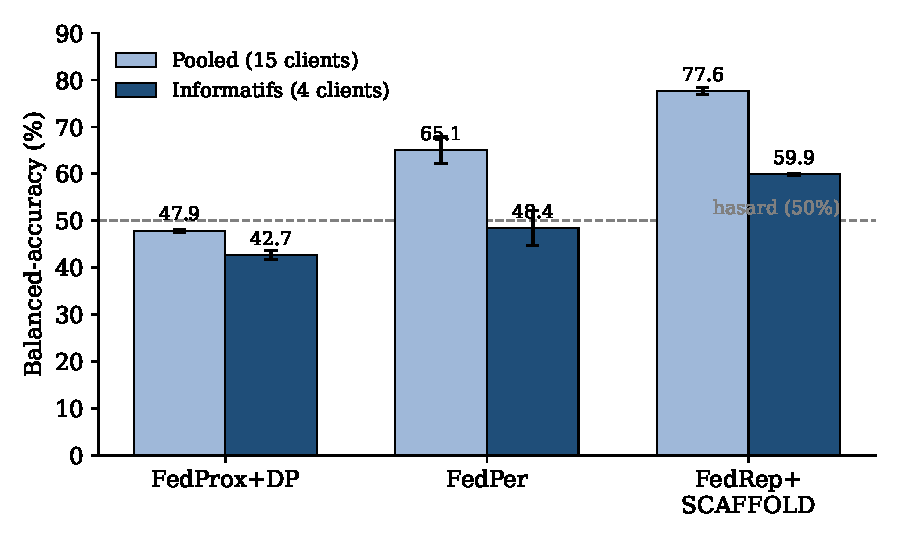
\includegraphics[width=0.8\linewidth]{fig_perso_comparison_full.pdf}
  \caption{Balanced-accuracy of the three architectures, pooled metric versus
  metric restricted to the 4 informative clients. The gap between the two bars of
  each pair directly measures the inflation caused by the 11 single-class
  clients.}
  \label{fig:perso_comparison}
\end{figure}

On the informative clients, the most clinically honest measure, the hierarchy
FedProx+DP $<$ FedPer $<$ FedRep+SCAFFOLD is statistically clear
(Figure~\ref{fig:perso_comparison}; Welch and Mann-Whitney on the 3 pairwise
comparisons, $p < 10^{-7}$ in every case, full detail in
\texttt{resultsfeat/fedper\_results\_summary.md}). Notably, FedProx+DP's AUC
drops to $0.20$ on these clients (worse than chance), confirming that the
aggregation problem identified in Section~\ref{subsec:why_cent_wins} is
precisely concentrated on the most heterogeneous clients. FedRep+SCAFFOLD is
also \textbf{markedly more stable} than the other two conditions on these
clients (balanced-accuracy standard deviation $0.22\,\%$ versus $3.65\,\%$ for
FedPer and $0.97\,\%$ for FedProx+DP). This was verified to be non-artefactual:
checkpoints from different seeds were compared directly and genuinely differ,
not a case of file recycling.

\paragraph{Limitation: non-negligible compute cost.} This grid required
$\approx$ 8.5 hours of compute (two full passes following the incident above),
versus $\approx$ 1.7 hours for FedProx+DP/FedPer, a factor $\approx 5\times$
slower per run, plausibly due to the non-vectorized SCAFFOLD correction loop
(Python iteration over parameters at every local step, up to $\approx 1240$
steps per round for the largest clients). Not rigorously profiled, but a real
compute cost not to be ignored, even outside any model-size constraint.

\subsection{Why Is the Privacy vs Utility Trade-off So Flat?}

Our results show a nearly constant balanced-accuracy across the whole tested
noise range (from $47.87\,\%$ at $\sigma=0.6$ to $48.12\,\%$ at $\sigma=1.8$, a
gap smaller than the inter-seed variance), while $\varepsilon$ varies by a factor
$\approx 10$ over this same range (Table~\ref{tab:epsilon_grid_extended}). Two
elements explain this flatness:

\begin{itemize}
  \item The personalization ablation (Section~\ref{subsec:ablation_personalization})
  shows that the global model itself remains stable as a function of $\sigma$
  ($77$--$78\,\%$ internal accuracy regardless of noise level): most of the
  privacy-related degradation is therefore already consumed at $\sigma = 0.6$,
  and increasing it further adds no measurable additional cost within the tested
  range.
  \item Gradient clipping ($C=1.0$) bounds each example's contribution
  independently of the noise level added afterward: it is this bound, more than
  the amplitude of the noise itself, that appears to dominate the learning
  dynamics on this small model and this feature set.
\end{itemize}

This finding is specific to the MLP Tiny architecture tested here and should not
be generalized beyond it without validation (see Limitations,
Section~\ref{subsec:synthesis}).

\subsection{Why Does INT8 Quantization Happen With Almost No Accuracy Loss Under
FL?}

Under the centralized regime, post-training dynamic quantization degrades
internal accuracy by $0.52 \pm 0.65\,\%$, whereas under FL + DP, the measured
degradation is nearly zero and even slightly negative on average
($\approx -0.05\,\%$, within measurement noise), meaning the INT8 quantized
version is sometimes marginally more accurate than the FP32 version it is
derived from.

This phenomenon is explained by the internal mechanics of
DP-SGD~\cite{abadi2016deep}. To bound data sensitivity, DP-SGD applies strict
\textbf{gradient clipping} ($C=1.0$) before injecting noise, which restricts how
fast parameters can evolve and acts as an implicit Tikhonov-style regularization
(\textit{weight decay}).

As shown in Figure~\ref{fig:dynamic_range}, this regularization sharply
compresses the weights' dynamic range compared to the centralized model. At
$\sigma = 0.8$, the FL + DP model's global dynamic range is $3.37 \pm 0.17$
(versus $9.45 \pm 1.03$ for the centralized model, a factor $\approx 2.8$), and
drops to $0.96 \pm 0.07$ on the first layer (versus $7.11 \pm 0.57$). Since the
FL model's weights are markedly more tightly clustered around zero, they spread
more uniformly across the 256-level INT8 quantization grid, suffering less
saturation or resolution loss than the centralized model's weights, whose wider
dynamic range is more heavily truncated by quantization.

\subsection{Why Does Peak RAM Usage Vary With Noise Level?}

The fluctuation in peak RAM observed during the call to \texttt{get\_epsilon()}
(from $11.34$~MB at $\sigma=1.8$ up to $33.65$~MB at $\sigma=0.6$) is a direct
consequence of Opacus's accounting algorithm~\cite{opacus}. Absent this call, the
memory footprint specific to the local training round remains stable and low
($\approx 0.18$~MB), regardless of noise level. Since the Opacus objects (engine,
optimizer, \textit{dataloader}) are instantiated once per client at the first
round and then reused (Section~\ref{subsec:dp}), most of the memory allocation
tied to data loading has already happened before round 30 and therefore no
longer appears in this peak measured at the end of the grid.

To compute the $\varepsilon$ budget, Opacus uses the PRV (\textit{Privacy Random
Variable}) approach by default. This algorithm performs a numerical evaluation of
the accumulated privacy-loss distribution (PLD) over the gradient history. The
lower the noise multiplier $\sigma$, the more concentrated this distribution
becomes. To maintain numerical precision during integration, the PRV algorithm
generates a much denser discrete grid, proportional to $1/\sigma$. It is this
temporary numerical grid that causes the observed RAM peak.

\subsection{Synthesis and Outlook}
\label{subsec:synthesis}

\subsubsection{Summary}

This work, built on a systematic grid search covering 25 federated runs
($\sigma \in [0.6;\, 1.8]$ over 5 seeds each) and several targeted ablations,
arrives at a result more fundamental than the FL-versus-centralized comparison
that was its starting point: \textbf{(0)~extreme heterogeneity across nurses
limits the generalization of every architecture tested, centralized included}.
11 of the 15 clients have a single-class test set (Section~\ref{subsec:dataset}),
which heavily distorts any 15-client pooled metric; restricted to the 4 clients
with a genuinely mixed test set, the most clinically honest measure, the
centralized model itself collapses (balanced-accuracy $45.73\,\%$, AUC $0.267$,
below chance, Section~\ref{subsec:why_cent_wins}), an underlying limitation
shared by every architecture, not a problem specific to FL. \textbf{Scope to
keep in mind}: the statistical significance of this gap ($p<10^{-4}$ in places)
is reproducible across seeds and noise levels, but structurally rests on only 4
clients with a mixed test set. This dataset offers no other one to check
generalization to a 5\textsuperscript{th} clinical profile
(Section~\ref{subsec:why_cent_wins}).

On this basis, this work shows that it is possible to build an operational FL
system that: (1)~provides a formal $(\varepsilon,
\delta)$-DP guarantee~\cite{dwork2014foundations} reaching $\varepsilon = 0.54 \pm 0.04$ at
$\sigma = 1.8$ (below $\varepsilon = 1$, a threshold commonly used in the DP
literature for sensitive applications); (2)~honestly quantifies, on both metrics
(pooled and informative clients), the cost of this privacy and decentralization
relative to a centralized baseline not deployable in practice on this type of
data: a gap of 10 points of balanced-accuracy on the pooled metric (57.84~\%
versus 47.9~\%) that shrinks to 3 points on the informative clients (45.73~\%
versus 42.73~\%), for a statistically equivalent raw accuracy in both cases
(82.0~\% versus 81.95~\%); (2bis)~decomposes this cost via a FedProx-without-DP-SGD
ablation (Table~\ref{tab:dp_decomposition}) and shows it is attributable
mainly to decentralization itself (FL without DP: $48.68\,\%$ pooled /
$45.18\,\%$ informative clients, versus $47.83\,\%$ / $42.73\,\%$ for FL+DP),
privacy noise adding only a secondary cost, more visible on the difficult
clients (2.45 points) than on the pooled metric (less than one point);
(3)~produces a model deployable on a microcontroller in 5.32~KB (FP32),
dynamically quantizable to INT8 with near-zero accuracy degradation, explained
by DP-SGD's gradient clipping, which sharply narrows the weights' dynamic range;
(4)~exhibits an empirically flat privacy/utility trade-off across the entire
tested range $\varepsilon \in [0.54;\, 5.29]$; (5)~tests an architecture that
removes aggregation of the classification layer (FedPer,
Section~\ref{subsec:fedper}): on the informative clients, balanced-accuracy rises
to $48.44 \pm 3.65\,\%$ (versus $42.73\,\%$ for standard FedProx+DP, +5.7 points,
statistically significant but modest in magnitude compared to the apparent
inflation on the pooled metric, +17.2 points), at the cost of a deployment
constraint specific to this architecture (no single global model, each client
keeps its own classification head); (5bis)~a complementary test isolating
granularity (Section~\ref{subsec:duration_vs_granularity}) shows that a simple
post-hoc fine-tuning of only the classification head, on the already-trained
standard FedProx+DP checkpoint and with no dedicated architecture, reaches
$55.88 \pm 2.35\,\%$, \textbf{more than FedPer itself}, without the dedicated
federated training path or the associated deployment constraint. This suggests
that most of the benefit does not come from the FedPer construction as such, but
from the possibility of lightly personalizing the head after the fact, a lead
probably simpler to deploy in practice; and (6)~pushes this logic further
outside the TinyML constraint (Section~\ref{subsec:fedrep_scaffold}) by
combining a multi-layer head, DP restricted to the extractor, and SCAFFOLD: on
the informative clients, the hierarchy FedProx+DP ($42.7\,\%$) $<$ FedPer
($48.4\,\%$) $<$ FedRep+SCAFFOLD ($59.9\,\%$, also markedly more stable) is
statistically clear, at the cost of a compute cost $\approx 5\times$ higher,
non-negligible even outside a model-size constraint. In every case, these
personalization architectures reduce the gap without ever eliminating it: even
FedRep+SCAFFOLD remains far from a fully satisfactory discriminative power on
the most atypical clients, consistent with finding (0) that the underlying
problem is heterogeneity itself, not just the choice of FL architecture. Point
(5bis) deserves to be retained as the most directly actionable result for a real
deployment: a lightweight post-processing step (freeze the extractor, fine-tune
the head on local data after receiving the standard global model) is enough to
obtain most of the personalization gain, with a markedly lower engineering load
than FedPer or FedRep+SCAFFOLD.

\subsubsection{Limitations and Future Work}
\label{subsec:synthesis_limits}

Several limitations deserve to be honestly reported:

\begin{itemize}
  \item \textbf{Model-size ablation to be replayed.} The ablation comparing MLP
  Tiny and MLP Medium has not yet been replayed on the current pipeline and is
  therefore not reported in this work.
  \item \textbf{$\delta$ slightly above the recommended threshold.} With the
  training set widened to $n = 306{,}886$ windows after label recombination,
  $\delta = 10^{-5}$ now exceeds the usual threshold $\delta < 1/n$ by a factor
  $\approx 3$ (Table~\ref{tab:dp_params_justif}). The reported $\varepsilon$
  values remain correctly computed for this $\delta$, but a $\delta = 10^{-6}$
  would be recommended for a future iteration.
  \item \textbf{Unreliable measurement of quantized model size.} The model-size
  computation function (\texttt{get\_model\_size}) enumerates parameters via
  \texttt{model.parameters()}, which does not cover the INT8 weights packed by
  \texttt{torch.quantization.quantize\_dynamic}. The effective INT8 size could
  therefore not be reliably measured in this work; only the theoretical
  compression factor ($\times 3.8$, Section~\ref{subsec:quantization}) is
  reported.
  \item \textbf{RAM measurement tied to the Opacus implementation.} Memory usage
  during the $\varepsilon$ computation depends heavily on the internal
  implementation of the PRV accountant~\cite{opacus}. Future work could
  implement an analytical accountant (based on the original \textit{moments
  accountant}~\cite{abadi2016deep}) to avoid this numerical overhead in a very
  constrained environment.
  \item \textbf{Single-node simulation.} Our evaluation was run as a simulation
  via Flower~\cite{beutel2020flower} on a single compute node. Validating real
  performance would require an actual decentralized deployment on physical
  wearables communicating over secure channels.
  \item \textbf{Cost of decentralization not yet reduced.} The only mitigation
  tested at global aggregation level (class-weighted loss,
  Section~\ref{subsec:why_cent_wins}) did not reduce the balanced-accuracy gap
  with the centralized model. Other leads (more informative physiological
  features, reweighting each client's contribution in FedProx aggregation,
  stronger personalization) were not explored in this work and constitute the
  natural continuation of this study. A more targeted lead, the best empirically
  supported among those listed here, emerges from the new-joiner scenario
  (Section~\ref{subsec:late_joiner_recall}): the optimal decision threshold after
  local adaptation diverges in opposite directions depending on the client
  ($0.001$ versus $0.950$ on the two tested cases), suggesting that a
  \emph{per-client} threshold calibration, performed on a dedicated validation
  split distinct from the test set, could bring a clinical recall gain without
  modifying the model itself, a lead that would be inexpensive to validate in a
  future iteration.
  \item \textbf{Results specific to this dataset and this configuration.} The
  measured cost of privacy, the near-zero quantization error, and the flatness
  of the privacy/utility trade-off are empirical observations specific to this
  Non-IID nurse-stress dataset and to this small MLP architecture. They should
  not be generalized without validation on other datasets and model sizes.
  \item \textbf{FedPer vs FedProx, duration and granularity: isolated
  separately, from the same checkpoint, with a paired statistical test.} The gap
  initially observed between FedPer and fine-tuned FedProx
  (Section~\ref{subsec:fedper}) could have reflected either the \emph{duration}
  of personalization or the \emph{granularity}. Isolated one after the other
  (Section~\ref{subsec:duration_vs_granularity}), each time starting from the
  same FedProx+DP checkpoint and with re-seeded fine-tuning (5 seeds, paired
  $t$-test): granularity dominates by far (+6.5 to +7.4 points, $p<0.03$,
  solidly established at 8 epochs, $p=6.2\times10^{-3}$, still an order of
  magnitude below the Bonferroni threshold adjusted for the 4 tests conducted,
  $\alpha=0.0125$). Personalizing only the head clearly outperforms fine-tuning
  the entire network, from an identical starting extractor, and duration also
  matters, more modestly (+1 to +2 points, $p<0.02$, both values surviving this
  same correction). Two successive corrections were needed to reach this
  result: a first test directly comparing FedPer (its own extractor) to
  FedProx's full fine-tuning confounded granularity with the fact that FedPer
  starts from an extractor trained under a different regime; a second test,
  correcting this point but without re-seeding the fine-tuning, had wrongly
  concluded that duration had no effect. Uncontrolled shuffling-order noise was
  masking a real but small effect. The paired Wilcoxon test plateaus at
  $p=0.0625$ on all four comparisons, a floor artifact specific to $n=5$
  same-sign pairs, not doubtful significance.
  \item \textbf{Domination of pooled metrics by single-class clients, corrected
  in this document, not merely documented.} Discovered during the evaluation of
  FedRep+SCAFFOLD (Section~\ref{subsec:fedrep_scaffold}): 11 of the 15 clients
  have a single-class test set (Section~\ref{subsec:dataset}), where a constant
  prediction mechanically achieves $100\,\%$ regardless of model quality. A
  systematic check was conducted on \emph{every} pooled table in this document
  (Tables~\ref{tab:main_results}, \ref{tab:dp_decomposition},
  \ref{tab:fedper_comparison}, \ref{tab:fedrep_scaffold_comparison}): each now
  reports the metric pooled over 15 clients \emph{and} the metric restricted to
  the 4 clients with a genuinely mixed test set (4, 5, 8, 12), the latter being
  the most clinically honest measure. The relative gaps between conditions
  remain qualitatively in the same direction on both metrics, but of markedly
  reduced magnitude on the informative metric for the centralized-vs-FL
  comparison (10 points $\to$ 3 points) and FedPer-vs-FedProx (17.2 points
  $\to$ 5.7 points). This is a change of magnitude, not merely a cosmetic
  adjustment, which motivated the reformulation of this document's central
  message (Section~\ref{subsec:why_cent_wins}).
\end{itemize}

\printbibliography

\end{document}
